% !TeX program = pdfLaTeX
\documentclass[smallextended]{svjour3}       % onecolumn (second format)
%\documentclass[twocolumn]{svjour3}          % twocolumn
%
\smartqed  % flush right qed marks, e.g. at end of proof
%
\usepackage{amsmath}
\usepackage{graphicx}
\usepackage[utf8]{inputenc}

\usepackage[hyphens]{url} % not crucial - just used below for the URL
\usepackage{hyperref}
\providecommand{\tightlist}{%
  \setlength{\itemsep}{0pt}\setlength{\parskip}{0pt}}

%
% \usepackage{mathptmx}      % use Times fonts if available on your TeX system
%
% insert here the call for the packages your document requires
%\usepackage{latexsym}
% etc.
%
% please place your own definitions here and don't use \def but
% \newcommand{}{}
%
% Insert the name of "your journal" with
% \journalname{myjournal}
%

%% load any required packages here




\usepackage{booktabs}
\usepackage{tabularx}
\usepackage{threeparttable}
\usepackage{bm}
\DeclareMathOperator{\Var}{Var}
\usepackage{dcolumn}
\usepackage{changepage}
\usepackage{lineno}
\linenumbers
\usepackage{booktabs}
\usepackage{longtable}
\usepackage{array}
\usepackage{multirow}
\usepackage{wrapfig}
\usepackage{float}
\usepackage{colortbl}
\usepackage{pdflscape}
\usepackage{tabu}
\usepackage{threeparttable}
\usepackage{threeparttablex}
\usepackage[normalem]{ulem}
\usepackage{makecell}
\usepackage{xcolor}

\begin{document}

\title{Sceptic priors and climate consensus \thanks{Estimate word count:
9,275. The data and source code for reproducing all of the results in
this paper can be found at the companion GitHub repository:
\url{https://github.com/grantmcdermott/sceptic-priors}} }



\author{  Grant R. McDermott \and  }


\institute{
        Grant R. McDermott \at
     Department of Economics, University of Oregon \\
     \email{\href{mailto:grantmcd@uoregon.edu}{\nolinkurl{grantmcd@uoregon.edu}}}  %  \\
%             \emph{Present address:} of F. Author  %  if needed
    \and
    }

\date{Received: date / Accepted: date}
% The correct dates will be entered by the editor


\maketitle

\begin{abstract}
How much evidence would it take to convince sceptics that they are wrong
about climate change? I explore this question within a Bayesian
framework. I consider a group of stylised sceptics and examine how these
individuals update their beliefs in the face of current and continuing
climate change. I find that available evidence in the form of
instrumental climate data tends to overwhelm all but the most extreme
priors. Most sceptics form updated beliefs about climate sensitivity
that correspond closely to estimates from the scientific literature.
However, belief convergence is a non-linear function of prior strength.
It thus becomes increasingly difficult to convince the remaining pool of
sceptics. I discuss necessary conditions for consensus formation under
Bayesian learning and show how apparent deviations from the Bayesian
ideal still be accommodated within the same conceptual framework. I
argue that a generalized Bayesian model thus provides a bridge between
competing theories of climate scepticism as a social phenomenon.
\\
\keywords{
        climate sceptics \and
        social cost of carbon \and
        Bayesian econometrics \and
    }


\end{abstract}


\def\spacingset#1{\renewcommand{\baselinestretch}%
{#1}\small\normalsize} \spacingset{1}


\hypertarget{sec:intro}{%
\section{Introduction}\label{sec:intro}}

Climate change has come to represent a defining policy issue of our age.
Yet support for comprehensive climate policy at the global scale remains
elusive. Many policy makers and citizens are openly sceptical about the
human role in our changing climate, despite decades of accumulated
research and an overwhelming scientific consensus
(\cite{oreskes2004beyond}, \cite{anderegg2010expert},
\cite{doran2011examining}, \cite{cook2013quantifying},
\cite{verheggen2014scientists}, \cite{tol2014quantifying},
\cite{cook2016consensus}, \cite{saad2019americans}). What are we to make
of this scepticism? And just how much evidence would it take to convince
climate sceptics that they are wrong? In the present paper, I seek to
answer these questions within a Bayesian framework that combines a range
of sceptic beliefs (i.e.~priors) with available climate data. My goal is
to pin down plausible rates of convergence with the scientific
consensus, by examining how different sceptics update their beliefs in
the face of current and continuing climate change. In so doing, I hope
to shed light on our current policy impasse and offer some remarks about
the possibility for finding common ground in the future.

Many studies have explored the cultural and psychological factors
underlying climate scepticism. These include \cite{kahan2011cultural},
\cite{kahan2012polarizing}, \cite{mccright2011cool},
\cite{mccright2011politicization}, \cite{corner2012uncertainty},
\cite{ranney2012changing}, \cite{clark2013knowledge},
\cite{lewandowsky2019influence} --- see \cite{hornsey2016meta} for a
recent literature review. My present concern is less with the origins of
scepticism than what it represents. Namely, a set of \emph{beliefs}
about the likely causes of global warming, which will in turn affect how
new information about those causes is interpreted. A convenient way to
model such beliefs is by defining scepticism in terms of climate
sensitivity, i.e.~the temperature response to a doubling of CO\(_2\).
Specifically, we can map sceptic beliefs directly on to subjective
estimates of climate sensitivity, because they both describe the likely
causes and probability distribution of future warming. The particular
measure of climate sensitivity that I focus on here is the transient
climate response (TCR). Formally, TCR describes the warming at the time
of CO\(_2\) doubling --- i.e.~after 70 years --- in a 1\% per year
increasing CO\(_2\) experiment \cite{ipcc2013i}. For the purposes of
this paper, however, it will simply be thought of as the contemporaneous
change in global temperature that results from a steady doubling of
atmospheric CO\(_2\).

According to the the Intergovernmental Panel on Climate Change
\cite{ipcc2013i}, TCR is ``likely'' to be somewhere in the range of
1.0--2.5 °C. This corresponds roughly to a 66--100\% probability
interval in IPCC terminology. The IPCC further emphasizes the inherently
Bayesian nature of climate sensitivity estimates, going so far as to
state:

\begin{quote}
\emph{{[}T{]}he probabilistic estimates available in the literature for
climate system parameters, such as ECS {[}i.e.~equilibrium climate
sensitivity{]} and TCR have all been based, implicitly or explicitly, on
adopting a Bayesian approach and therefore, even if it is not explicitly
stated, involve using some kind of prior information.}
\cite[p. 922]{ipcc2013i}
\end{quote}

To understand why classical (i.e.~frequentist) methods are ill-suited
for the task of producing credible estimates of climate sensitivity,
recall that frequentism interprets probability as the limiting frequency
in a large number of repeated draws. Such a narrow definition holds
little relevance to the question of climate sensitivity, for which there
exists but one unique value. There is no population of ``sensitivities''
to draw samples from. I also adopt a Bayesian framework to determine
climate sensitivity and its concomitant policy implications. However, my
approach differs from the previous literature along several dimensions.

The most obvious point of departure is the fact that I deliberately
focus on the beliefs of sceptics. Priors for determining climate
sensitivity are usually based on paleo data, the judgments of scientific
experts, or noninformative methods. Such approaches may possess obvious
scientific merit for establishing a best estimate of climate
sensitivity. Yet, they are of limited relevance for understanding
people's motivations and voting behaviour when it comes to actual
climate policy. My approach is to take sceptics at their word and work
through to the conclusions of their stated priors. In other words, my
goal is to recover posterior probabilities about the rate and causes of
climate change that are logically consistent with the initial beliefs of
these sceptics.

Contrarian climate beliefs have also been largely ignored in the
economic policy literature to date. The handful of studies that do
consider policy options from the sceptic perspective have tended to
emphasise edge scenarios like climate catastrophe and irreversibility.
For example, \cite{kiseleva2016heterogeneous} introduces an IAM of
heterogeneous agents that incorporates various degrees of climate
scepticism. She shows that a world comprised only of sceptical policy
makers will make sufficient investments in mitigation measures to avoid
catastrophic outcomes. The key mechanism is a dominant subset of
``weak'' sceptics who are sufficiently concerned by anthropogenic
climate change that they reduce their emissions accordingly.
\cite{kiseleva2016heterogeneous} does not allow for learning in her
simulations.\footnote{It should be said that there \emph{is} an
  important literature on Bayesian learning in IAMs that originates with
  \cite{kelly1999learning}. But I am not aware of any study that
  attempts to integrate learning by climate sceptics into an IAM.}
However, theoretical work by \cite{wijnbergen2015skeptics} show that
climate sceptics actually have an incentive to reduce emissions, since
it will facilitate learning about the true causes of climate change.
While it is possible for an increase in emissions to yield similar
learning effects, the irreversibility of climate change renders this an
inferior strategy. From a methodological perspective, the present paper
differs from these earlier studies by combining Bayesian learning with
an empirical framework.\footnote{In terms of tangentially related
  empirical work, \cite{kaufmann2017spatial} shows that spatial
  heterogeneity in local climate change effects and temperatures can
  partially explain persistent scepticism in different regions of the
  United States. \cite{moore2017learning} does not deal with sceptics
  \emph{per se}, but characterises learning about climate as a
  (potentially) Bayesian process where individuals make inferences based
  on local weather shocks. This builds off of earlier work by
  \cite{deryugina2013update}, who finds that longer spells of abnormal
  local weather patterns are consistent with Bayesian updating about
  climate beliefs.}

Unlike the existing numerical and game-theoretic approaches, described
above, I am not attempting to prescribe an optimal emissions strategy or
learning paths for climate sceptics under future uncertainty. Rather, my
goal is to establish some ground rules for thinking about climate policy
today, given the information that is already available to us.

Another distinguishing feature of this paper is that the results are
derived via conceptually straightforward time-series regression
analysis. While climate scientists have typically relied on complex
computer models to simulate TCR, a growing body of research is aimed at
understanding the link between human activities and climate change
through the purview of time-series econometrics. Much of this literature
has concerned itself with the apparent non-stationarity of climate data
over time. The present paper takes as its foundation recent research
(\cite{gay2009global}, \cite{estrada2013statistically},
\cite{estrada2013time}, \cite{kim2020inference}), which argues
convincingly that global surface temperatures and anthropogenic forcings
are best described as trend-stationary processes, incorporating common
structural breaks.\footnote{Another group of researchers beginning with
  \cite{stern2000detecting}, has argued that the instrumental
  temperature record contains a stochastic trend that is imparted by,
  and therefore cointegrates with, the time-series data of radiative
  forcings. The reader is referred to \cite{estrada2013detection} and
  \cite{hillebrand2020econometric} for a helpful overviews of this
  debate.} The upshot is to permit the use of level terms within an
ordinary least squares (OLS) regression framework. Such matters
notwithstanding, virtually all econometric studies of climate change
attribution to date have been carried out in the frequentist paradigm.
They do not consider the influence of priors, nor are they able to yield
the probabilistic estimates that are characteristic of Bayesian
analysis. A noteworthy and early exception is that of
\cite{tol1998bayes}, who are motivated to adopt a Bayesian approach
because of multicollinearity in their anthropogenic emissions data. Such
multicollinearity does not plague newer datasets, since these are
defined in common units as will be discussed in Section \ref{sec:data}.
Further, \cite{tol1998bayes} do not consider the influence of overtly
contrarian priors as a basis for affecting policy.

\hypertarget{sec:econometric}{%
\section{Econometric approach}\label{sec:econometric}}

\hypertarget{sec:bayesian}{%
\subsection{Bayesian regression overview}\label{sec:bayesian}}

The Bayesian regression framework is less familiar to many researchers
than the frequentist paradigm that is commonly taught in universities.
For this reason, I provide a brief overview of the key principles of the
Bayesian method and highlight some important distinctions versus the
frequentist approach.

A Bayesian regression model uses the logical structure of Bayes' theorem
to estimate probable values of a set of parameters \(\theta\), given
data \(X\):

\begin{equation}
    p(\theta|X) = \frac{p(X|\theta)p(\theta)}{p(X)}. \label{eq:bayes}
\end{equation}

Here, \(p(\theta|X)\) is known as the \textit{posterior} and serves as
the fundamental criterion of interest in the Bayesian framework. The
posterior asks, ``What are the probable values of our parameters, given
the observed data?'' This stands in direct contrast to the first term in
the right-hand numerator, \(p(X|\theta)\), which is the familiar
\textit{likelihood function} from frequentist statistics. The likelihood
essentially reverses the question posed by the posterior and instead
asks, ``How likely we are to observe some data for a given set of
parameters (e.g.~based on an assumption about the data generating
process)?'' The second term in the numerator is the \textit{prior},
\(p(\theta)\). While the prior can take on any distributional form, it
should in principle encapsulate our knowledge about the parameters
before we have observed the data. Insofar as we are interested in
learning about \(\theta\), it is common practice to ignore the term in
the denominator, \(p(X)\). This is simply the marginal probability of
the data and can be thought of as a normalisation constant, which helps
to ensure that the posterior is a proper probability distribution
(i.e.~integrates to one) and can be calculated \textit{ad hoc} if
needed. For this reason, eq.(\ref{eq:bayes}) is typically re-written as

\begin{equation}
    p(\theta|X) \propto p(X|\theta)p(\theta). \label{eq:bayesprop}
\end{equation}

Equation (\ref{eq:bayesprop}) embodies the mantra of Bayesian
statistics: ``The posterior is proportional to the likelihood times the
prior.'' Solving for the posterior typically involves the combination of
various integrals, which cannot be calculated analytically.\footnote{A
  famous exception is that of conjugate priors, which belong to the same
  distribution family as the resulting posterior. However, this places
  strong restrictions on the questions that can asked of the data.}
Fortunately, we can simulate the posterior density computationally using
Markov Chain Monte Carlo (MCMC) routines. This can be done for virtually
any combination of prior and likelihood function. Obtaining a valid
posterior is then simply a matter of: (i) choosing a prior distribution
for our regression parameters, i.e.~regression coefficients and
variances; and (ii) specifying a likelihood function to fit the data.
For ease of exposition --- how we map parameter values to beliefs about
TCR will be determined by the specification of the regression model ---
I begin with the likelihood function.

\hypertarget{sec:likelihood}{%
\subsection{Likelihood function}\label{sec:likelihood}}

The likelihood function is governed by the choice of empirical model.
Following \cite{estrada2012breaks} and \cite{estrada2013statistically},
I model global temperatures using the regression equation

\begin{equation}
   GMST_t = \alpha_0 + \beta_1RF_t + \gamma_2VOLC_t + \delta_3SOI_t + \eta_4AMO_t + \epsilon_t, \label{eq:regression}
\end{equation}

where \(\epsilon_t = \phi \epsilon_{t-1} + \nu_t\) is a first-order
autoregressive, or AR(1), error process.

Here, \(GMST\) is the global mean surface temperature anomaly relative
to the pre-industrial period (defined as the 1871--1900 average); \(RF\)
is total radiative forcing due to both anthropogenic and natural factors
(excluding volcanic eruptions); \(VOLC\) is the radiative forcing due to
volcanic stratospheric aerosols; and \(SOI\) and \(AMO\) are scaled
indices of these respective climatic phenomena. The subscript \(t\)
denotes time. Specifying that the error term \(\epsilon\) follows an
AR(1) process allows us to account for dynamic elements such as
potential autocorrelation.

Two points merit further discussion before continuing. First, nothing
much hinges on the use of OLS for estimating TCR. For example, the
\(\beta_1\) coefficient above is equivalent to the ``climate
resistance'' constant (\(\rho\)) described in
\cite{gregory2008transient}; a point I shall return to later. OLS simply
provides a convenient method for combining data and priors in a
consistent Bayesian framework. Other methods could in principle be used
to derive the same results. Second, the use of a composite \(RF\)
variable that combines both anthropogenic and natural forcings may, at
first blush, seem an odd choice. After all, the goal of this paper is to
separate out and interrogate scepticism specifically about the human
role in climate change. However, recall that the underlying forcings in
my dataset are all expressed in terms of a common unit
(i.e.~Wm\(^{-2}\)). This circumvents the multicollinearity problems that
would arise from estimating an econometric model on forcings that have
been separated out.\footnote{Anthropogenic forcings such as CO\(_2\),
  CH\(_4\), and N\(_2\)O all follow very similar trends over time. Any
  empirical model that does not constrain these forcings in some way
  will therefore struggle to correctly attribute warming between them.}
Econometric issues aside, the use of a common forcing unit ensures that
I don't run the risk of estimating different coefficients, which would
imply an inconsistent response of the climate system to identical
forcings. The use of a composite forcing series is thus a necessary step
to ensure that the model remains physically consistent.\footnote{Volcanic
  aerosols are an exception because they impart only a transitory level
  of forcing. This explains why \(VOLC\) may be included as a separate
  component in the regression equation \cite{estrada2013statistically}.}
Nonetheless, I show in an alternate specification later in the paper
that relaxing this constraint leads to near identical conclusions as the
physically correct specification. I also show that the core results do
not hinge on the imposition of a common efficacy among different forcing
agents.

Returning to my primary regression model, eq. (\ref{eq:regression})
implies a likelihood function that is multivariate normal

\begin{equation}
   p(GMST | \boldsymbol{\beta}, \sigma^2) =  \frac{1}{\left(2 \pi \sigma^2\right)^{T/2}} \text{exp}\left[ - \frac{(GMST - \mathbf{X}\boldsymbol{\beta})'(GMST - \mathbf{X}\boldsymbol{\beta})}{2 \sigma^2} \right], \label{eq:likelihood}
\end{equation}

where \(\mathbf{X}\) is the design matrix of explanatory variables;
\(\boldsymbol{\beta}\) is the coefficient vector;
\(\sigma^2 = \mathop{\mathrm{Var}}(\epsilon)\) is the variance of the
error term; and \(T=140\) is the number of years in the collated,
historical dataset. Eq. (\ref{eq:likelihood}) can also be written more
simply as
\(GMST | \boldsymbol{\beta}, \sigma^2 \sim \mathcal{N}_T(\mathbf{X}\boldsymbol{\beta}, \sigma^2\mathbf{I})\).

An important feature of eqs. (\ref{eq:regression}) and
(\ref{eq:likelihood}) is that they define how we should map
probabilities about the regression parameters to beliefs about climate
sensitivity. Recall that TCR describes the contemporaneous change in
temperature that will accompany a steady doubling of atmospheric
CO\(_2\) concentrations. It follows that

\begin{equation}
   \text{TCR} = \beta_1 * F_{2\times}\ , \label{eq:impliedtcr}
\end{equation}

where \(\beta_1\) is the regression coefficient describing how
responsive global temperatures are to a change in total radiative
forcing, and \(F_{2\times}\) is the change in forcing that results from
a doubling of CO\(_2\). For the latter, I use the IPCC's best estimate
of \(F_{2\times}=3.71 \text{ Wm}^{-2}\) and further assume an additional
\(\pm10\%\) variation to account for uncertainties over spatial
heterogeneity and cloud formation (\cite{schmidt2007co2} and
\cite{ipcc2001i}).\footnote{It is worth noting that a number of studies
  which provide climate sensitivity estimates via time-series methods
  --- e.g.~\cite{kaufmann2006emissions}, \cite{mills2009robust},
  \cite{estrada2012breaks} --- do so under the assumption that
  \(F_{2\times}=4.37 \text{ Wm}^{-2}\). This outdated figure appears to
  be based on early calculations by \cite{hansen1988global}. The climate
  sensitivity estimates of these studies may consequently be regarded as
  inflated.} The key point is that assigning a distribution over the
parameter \(\beta_1\) will necessarily imply a distribution for TCR, and
vice versa. We therefore have a direct means of linking prior and
posterior probabilities of the regression parameters to beliefs about
TCR. It also means that the primary goal of the regression analysis will
be to determine probable values of \(\beta_1\). The rest of the
parameters will take a backseat in the analysis that follows, acting
largely as controls.

Eq. (\ref{eq:impliedtcr}) contains an implicit assumption that will have
bearing on the external validity of my results --- specifically, the
extent to which they can be extrapolated to different future climate
scenarios. Recall, as stated earlier, that \(\beta_1\) is equivalent to
the ``climate resistance'' parameter (\(\rho\)) defined in
\cite{gregory2008transient} as the constant sum of the ocean heat uptake
efficiency and the climate feedback parameter. The importance of this
equivalence is that it underscores the role of oceanic thermal dynamics
in assuming a linear scaling between the different climate components of
my regression model. While the linear relationship holds for scenarios
where radiative forcing increases at steady rates --- as was true for
the historical period under consideration --- it cannot be expected to
do so in scenarios that overturn it. In such cases, ocean heat uptake
would need to be modeled separately to account for inertia in the
climate system and its resultant impact on GMST (\emph{ibid}.). All of
which is to say that I will limit my analysis to the historical period,
as well as future climate scenarios that are characterised by steady
increases in radiative forcing.

\hypertarget{sec:priors}{%
\section{Priors}\label{sec:priors}}

\begin{table}[t] \centering 
    \caption{Sceptic priors} 
    \label{tab:sceppriors} 
    \begin{threeparttable} 
        %\begin{tabular}{@{\extracolsep{5pt}} lcc} 
        \begin{tabular}{@{\extracolsep{0pt}}lD{,}{,}{-3} D{,}{,}{-3}}
            \toprule
            \multicolumn{1}{l}{Type}                & \multicolumn{1}{c}{TCR ($^\circ$C)} & \multicolumn{1}{c}{Implied $\beta_1$} \\ 
            \midrule
            \multicolumn{1}{l}{Moderate lukewarmer} & \mathcal{N}(1, \ 0.25^2)           & \mathcal{N}(0.27, \ 0.0674^2)         \\
            \multicolumn{1}{l}{Strong lukewarmer}  & \mathcal{N}(1, \ 0.065^2 )          & \mathcal{N}(0.27, \ 0.0175^2)         \\
            \multicolumn{1}{l}{Moderate denier}    & \mathcal{N}(0, \ 0.25^2)           & \mathcal{N}(0, \ 0.0674^2)            \\
            \multicolumn{1}{l}{Strong denier}       & \mathcal{N}(0, \ 0.065^2)           & \mathcal{N}(0, \ 0.0175^2)            \\ 
            \midrule
            \multicolumn{1}{l}{Noninformative}       &  -           & \mathcal{N}(0, \ 1.214^2) \\
            \bottomrule
        \end{tabular} 
        \begin{tablenotes}
            \footnotesize
            \item \textit{Notes:} Subjective priors types are defined according to the mean (Lukewarmer vs Denier) and variance (moderate vs strong) parameters of normal distributions over TCR. The implied priors for $\beta_1$ are obtained using the simple formula described in eq. (\ref{eq:impliedtcr}), i.e. $\beta_1 = \text{TCR}/3.71$. The noninformative prior presented at the bottom of the table is weakly data-dependent (i.e. depends on the scale of the data) and is obtained using the default calculation proposed by \cite{rstanarm}, $\beta_1 \sim \mathcal{N}(0, \ 2.5 \cdot \text{sd}(GMST) / \text{sd}(RF))$. See text for details.\\
        \end{tablenotes}
    \end{threeparttable} 
\end{table}

Climate scepticism is a matter of degree. I account for this fact by
defining a simple typology of sceptics as per Table
\ref{tab:sceppriors}. Summarizing, I distinguish between two basic
sceptic archetypes based on their best guess for TCR.
\textit{Lukewarmers} believe that TCR lies around 1 \(^\circ\)C ---
i.e.~the lower bound of the IPCC likely range (c.f.
\cite{ridley2015lukewarmer}) --- while \textit{deniers} believe that TCR
is likely zero. I further distinguish these individuals based on how
certain they are about their best guess. A person with \textit{moderate}
convictions believes that the true value of TCR lies within a 1
\(^\circ\)C uncertainty interval of their prior mean (95\% probability),
while that interval falls to just 0.25 \(^\circ\)C for someone with
\textit{strong} convictions. Altogether this yields a spectrum of
sceptic priors that ranges from moderate lukewarmers to strong deniers.
Importantly, each sceptic can all be represented mathematically by a
prior distribution on TCR. I assume normal distributions for simplicity,
where the mean represents an individual's best guess and the variance
their uncertainty.\footnote{The choice of normally-distributed priors
  should have little bearing on the generality of the results. An
  exception might occur if I assumed a bounded prior, like a triangular
  or uniform distribution. Because these bounded distributions assign
  zero weight to outcomes beyond a specific interval, no amount of data
  can shift the posterior beyond that interval. This idea, that a
  Bayesian posterior can converge on a particular outcome only if the
  prior allocates some (infinitesimal) weight to it, is known
  colloquially as \emph{Cromwell's rule} (\cite{jackman2009bayesian}).}
Following eq. (\ref{eq:impliedtcr}), obtaining priors over \(\beta_1\)
is a simple matter of dividing the respective TCR distributions by
\(F_{2\times}=3.71\text{ Wm}^{-2}\). These are the parameters that
actually enter the Bayesian regression model and are also shown in Table
\ref{tab:sceppriors}.

In addition to the subjective priors of our stylised sceptics, a useful
reference case for the analysis is provided by a set of so-called
\emph{noninformative} priors. Loosely speaking, noninformative priors
are vague and should not privilege particular parameter values over
others. In practice, however, applied Bayesian researchers are advised
to use noninformative priors that are weakly data-dependent
(\cite{gelman2020regression}). For example, priors should be scaled to
reflect feasible magnitudes of the underlying data. If the data are
observed in the order of millimeters, then the prior should not allocate
plausible weight to values in the order of kilometers, etc. This modest
form of regularisation not only helps to ensure computational stability,
but also avoids some of the theoretical pathologies associated with
uniform priors (c.f. \cite{annan2009probabilistic}). I therefore use a
set of reference priors that have been scaled to reflect this limited
data dependence. Specifically, given generic dependent variable \(y\)
and independent variable \(x\), I define a noninformative prior for the
associated regression coefficient
\(\beta_x \sim \mathcal{N}(0, \ 2.5 \frac{s_y}{s_x})\), where
\(s_x = \text{sd}(x)\).\footnote{This is the default prior suggested by
  \cite{rstanarm}, which they refer to as ``weakly informative''.} In
other words, my noninformative priors take the form of normal
distributions with wide variances. For my default regression
specification this equates to a prior on the key radiative forcing
coefficient of \(\beta_1 \sim \mathcal{N}(0, \ 1.214^2)\).

Note that my group of sceptics only hold subjective priors over TCR (and
thus \(\beta_1\)). Noninformative priors are always assumed for the
remaining parameters in the regression equation. Similarly, I
acknowledge that these sceptics are, of course, highly stylised
caricatures. Their priors are simply taken as given. I am not concerned
with where these priors come from and why they are of a particular
strength. However, such abstractions are ultimately unimportant given
the objectives of this study. My goal is to explore how climate sceptics
would respond to evidence for climate change, provided that they update
their beliefs rationally. Moreover, it gives a sense of just how strong
someone's prior beliefs need to be, so as to preclude the acceptance of
any policy interventions.

\hypertarget{sec:data}{%
\section{Data}\label{sec:data}}

\begin{table}[t]
    \caption{Data sources}
    \label{tab:sources}
    \small
    \centering
    \begin{threeparttable}
        \begin{tabularx}{\linewidth}{ l l X l}
            \toprule
            Variable    & Key & Description & Period \\
            \midrule
            GMST    &   HadCRUT4$^\text{a}$ &   Global mean surface temperature. Primary series. Compiled by the UK Met Office and the Climatic Research Unit at the University of East Anglia. & 1850--2019 \\
                        &   CW14$^\text{b}$     &   Secondary series. Compiled by \cite{cowtan2014coverage}. Corrects for coverage bias in HadCRUT4.    & 1850--2019 \\
                        & GISTEMP$^\text{c}$        & Secondary series. Compiled by the NASA Goddard Institute for Space Studies.                                           &   1880--2015 \\
            \midrule
            RF      & RCP$^\text{d}$                & Total radiative forcing due to anthropogenic and natural factors (excluding volcanic aerosols). Compiled by \cite{meinshausen2011rcp}. Historical data until 2005, simulated scenarios thereafter.                & 1765--2300 \\
                    & DF18$^\text{e}$               & Ensemble of 1,000 radiative forcing estimates compiled by \cite{dessler2018ecs}. Used for sensitivity analysis.               & 1750--2017 \\
            \midrule
            VOLC        & RCP$^\text{d}$                & Radiative forcing due to volcanic stratospheric aerosols. Compiled by \cite{meinshausen2011rcp}.                                                                                          & 1750--2005 \\
            \midrule
            AMO     & NOAA$^\text{f}$               & Atlantic Multidecadal Oscillation.                                            &   1856--2019 \\
            SOI     & NCAR$^\text{g}$               & Southern Oscillation Index.                                                           &   1866--2019 \\
            \bottomrule
        \end{tabularx}
    \begin{tablenotes}
        \footnotesize
            \item \textit{Notes:} The compiled dataset, as well as the code needed to reconstruct from source, are available at \url{https://github.com/grantmcdermott/sceptic-priors}. Sources are listed below.
            \item $^\text{a}$ \url{http://www.metoffice.gov.uk/hadobs/hadcrut4/data/current/download.html}
            \item $^\text{b}$ \url{http://www-users.york.ac.uk/~kdc3/papers/coverage2013/series.html} 
            \item $^\text{c}$ \url{http://data.giss.nasa.gov/gistemp}
%           \item $^\text{d}$ \url{http://www.iiasa.ac.at/web-apps/tnt/RcpDb} 
            \item $^\text{d}$ \url{http://www.pik-potsdam.de/~mmalte/rcps} 
            \item $^\text{e}$ \url{https://doi.org/10.5281/zenodo.1323162}, (original) \url{https://github.com/hausfath/OldModels} (accessed)
            \item $^\text{f}$ \url{http://www.esrl.noaa.gov/psd/data/timeseries/AMO}
                \item $^\text{g}$ \url{http://www.cgd.ucar.edu/cas/catalog/climind/soi.html}        
            \end{tablenotes}
    \end{threeparttable} 
\end{table}

The various data sources for this paper are summarised in Table
\ref{tab:sources}. Global mean surface temperature data (1850--2017) are
taken from the HadCRUT4 dataset, jointly compiled by the UK Met Office
and the Climatic Research Unit at the University of East Anglia. Two
alternate global temperature reconstructions --- one provided by
\cite{cowtan2014coverage} and the other by the NASA Goddard Institute
for Space Studies (GISTEMP) --- are used as a check against coverage
issues and other uncertainties. Radiative forcing data, covering both
historic estimates (1765--2005) and future scenarios (2006-2300), are
taken from the Representative Concentration Pathway (RCP) database,
hosted by the Potsdam Institute for Climate Impact Research. These data
include anthropogenic sources of radiative forcing like industrial
greenhouse gas emissions, as well as natural sources like solar
irradiance and volcanic eruptions. As a part of the sensitivity
analyses, I use an ensemble of 1,000 forcing estimates to capture
measurement uncertainty about radiative forcing data. This ensemble
originates with \cite{dessler2018ecs}, although I use a recapitulated
version provided by \cite{hausfather2020evaluating} for ease of access.
Data for two major oceanic-atmospheric phenomena, the Atlantic
Multidecadal Oscillation (AMO, 1856--2017) and the Southern Oscillation
Index (SOI, 1866--2017), are taken from the U.S. National Oceanic and
Atmospheric Administration (NOAA) and National Center for Atmospheric
Research (NCAR). Summarising the common historic dataset for which data
are available across all series, we have 140 annual observations running
over 1866--2005. RCP scenarios until 2100 will also be considered for
making future predictions later in the paper.

\hypertarget{sec:results}{%
\section{Results}\label{sec:results}}

The analysis for this project was primarily conducted in \texttt{R}
(\cite{rcore}, version 4.0.2), with the Bayesian computation being
passed on to the \texttt{Stan} programming language (\cite{cmdstanr}).
All of the code and data needed to reproduce the results can be found at
the companion GitHub repository.\footnote{\url{https://github.com/grantmcdermott/sceptic-priors}.}

\hypertarget{sec:regression}{%
\subsection{Regression results and updated TCR
beliefs}\label{sec:regression}}

The posterior regression results for the various prior types are
presented in Table \ref{tab:reg}. Each column contains the results from
running the Bayesian regression eq. (\ref{eq:regression}) over the full
historical data set (1866--2005), using a particular set of priors.
Beginning with the noninformative case in the first column, all of the
regression coefficients are credibly different from zero and of the
anticipated sign. For example, GMST is negatively correlated with SOI.
This is to be expected since the El Niño phenomenon is defined by SOI
moving into its negative phase. The posterior coefficient density on our
main parameter of interest, total radiative forcing (\(RF\)), shows that
global temperature will rise by an average of 0.426 °C for every
Wm\(^{-2}\) increase. Of greater interest, however, is the fact that the
posterior estimates yielded by the group of sceptic priors are very
similar to this noninformative case. With the exception of the Strong
Denier, there is a clear tendency to congregate towards the
noninformative parameter values.

\begin{table}

\caption{\label{tab:regtab}Regression results and implied TCR \label{tab:reg}}
\centering
\fontsize{8}{10}\selectfont
\begin{threeparttable}
\begin{tabular}[t]{lccccc}
\toprule
\multicolumn{2}{c}{ } & \multicolumn{2}{c}{Lukewarmer} & \multicolumn{2}{c}{Denier} \\
\cmidrule(l{3pt}r{3pt}){3-4} \cmidrule(l{3pt}r{3pt}){5-6}
 & Noninformative & Moderate & Strong & Moderate & Strong\\
\midrule
RF & 0.426 & 0.417 & 0.345 & 0.402 & 0.076\\
 & (0.395, 0.455) & (0.387, 0.448) & (0.317, 0.373) & (0.371, 0.433) & (0.040, 0.112)\\
VOLC & 0.048 & 0.048 & 0.046 & 0.047 & 0.034\\
 & (-0.002, 0.098) & (-0.000, 0.097) & (-0.013, 0.102) & (-0.006, 0.097) & (-0.080, 0.148)\\
SOI & -0.024 & -0.024 & -0.025 & -0.024 & -0.025\\
\addlinespace
 & (-0.035, -0.012) & (-0.035, -0.013) & (-0.038, -0.014) & (-0.036, -0.013) & (-0.044, -0.006)\\
AMO & 0.470 & 0.468 & 0.460 & 0.468 & 0.448\\
 & (0.393, 0.548) & (0.386, 0.547) & (0.367, 0.552) & (0.386, 0.549) & (0.289, 0.614)\\
\midrule
AR(1) & 0.320 & 0.321 & 0.378 & 0.326 & 0.648\\
 & (0.181, 0.444) & (0.187, 0.446) & (0.245, 0.503) & (0.194, 0.454) & (0.549, 0.733)\\
\midrule
\addlinespace
TCR & 1.6 & 1.5 & 1.3 & 1.5 & 0.3\\
 & (1.4, 1.8) & (1.4, 1.7) & (1.1, 1.4) & (1.3, 1.7) & (0.1, 0.4)\\
\bottomrule
\end{tabular}
\begin{tablenotes}[para]
\item \textit{Notes:} 
\item Results from running the Bayesian regression eq. (\ref{eq:regression}). The table lists the posterior parameter means, with 95\% Bayesian credible intervals in parentheses. Models are distinguished by the set of priors that were used during the Bayesian estimation. For the first model in column (1), noninformative priors were specified over all regression parameters. For the remaining models in columns (2)--(5), subjective priors were specified over the total radiative forcing (RF) coefficient, with noninformative priors being used for all other parameters. See Table \ref{tab:sceppriors} for details. RF and volcanic stratospheric aerosols (VOLC) are measured in Wm$^{-2}$. The Southern Oscillation Index (SOI) and Atlantic Multidecadal Oscillation (AMO) are measured as scaled indices. The AR(1) term denotes an autoregressive error coefficient. The implied TCR values at the bottom of the table are measured in °C and are obtained by multiplying the coefficient on RF by $F_{2\times}$ per eq. (\ref{eq:impliedtcr}). The data have been centered, hence the lack of intercept, and comprise annual observations over 1866--2005.
\end{tablenotes}
\end{threeparttable}
\end{table}

Of course, the exact values of the regression parameters are themselves
of somewhat limited interest. Rather, their primary usefulness is to
enable the recovery of posterior beliefs about TCR. These are summarised
at the bottom of Table \ref{tab:reg}, while the full prior and posterior
distributions are plotted in Fig. \ref{fig:tcrs-dens}. We see that the
posterior TCR distributions are generally clustered around a best
estimate of 1.5 °C, with a 95\% credible interval in the region of
1.1--1.8 °C, depending on the prior. Excepting the Strong Denier, these
posterior beliefs about TCR fall comfortably within the IPCC ``likely''
range. However, the derived probability intervals are decidedly narrower
and TCR values at the upper end of the spectrum are discounted
accordingly.

\begin{figure}

{\centering 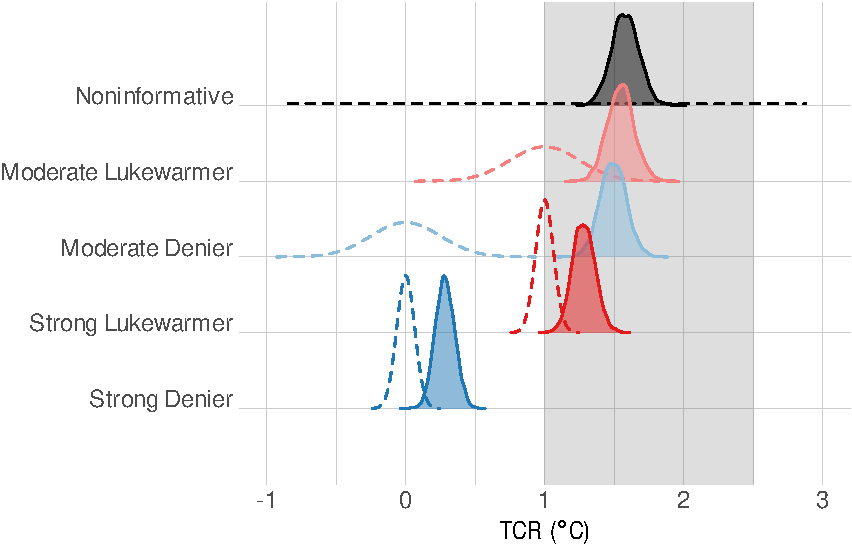
\includegraphics[width=1\linewidth]{/home/grant/Documents/Papers/Sceptic/sceptic-priors/figs/tcrs-dens-1} 

}

\caption{TCR densities. Dashed lines denote priors, solid lines denote posteriors. The grey shaded region denotes the IPCC "likely" TCR range of 1.0--2.5 °C.}\label{fig:tcrs-dens}
\end{figure}

Further insight into the updating behaviour of our stylised sceptics is
provided by the recursive TCR estimates shown in Fig.
\ref{fig:recursive}. It is apparent that stronger convictions about
one's prior beliefs (in the form of a smaller prior variance) have a
greater dampening effect on posterior outcomes than the prior mean. For
example, the Moderate Denier converges more rapidly to the
noninformative distribution than the Strong Lukewarmer. However, most
sceptics will converge to the noninformative distribution only after
``observing'\,' data from a number of decades. Note that this does not
alter the conclusions that we are able to draw from our Bayesian
analysis. As long as we have fully specified a prior that encapsulates a
person's initial beliefs, then we should in principle treat the full
historical dataset as new information for updating those
beliefs.\footnote{As a corollary, concerns over the use of the full
  historical dataset would only hold sway in cases where priors already
  incorporate information that has been obtained from applying the same
  model on a sub-sample of the dataset. In that case, we would need to
  exclude the sub-sample from the analysis to derive a valid posterior
  that avoids double counting.} Yet it does highlight the importance of
using all the available instrumental climate data for building any kind
of policy consensus. Limiting the sample period under observation to,
say, the last 35 years would largely preclude the possibility of
consensus formation. The tendency of some prominent sceptics to rely on
satellite records of global temperatures --- which only stretch back as
far as 1979 --- could be seen as anecdotal evidence in support of this
claim (e.g.~\cite{mooney2016cruz}). A similar argument could be made for
a reliance on short-term climate trends and fluctuations that do
accurately reflect longer-term trends. For example, the relatively brief
``hiatus'' in warming that followed the exceptionally strong 1998 El
Niño event (\cite{lewandowsky2016pause}).

\begin{figure}

{\centering 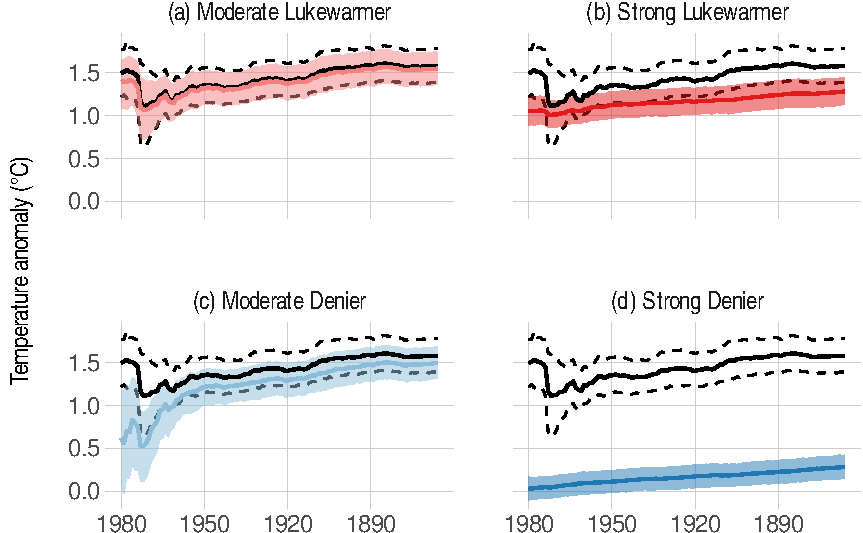
\includegraphics[width=1\linewidth]{/home/grant/Documents/Papers/Sceptic/sceptic-priors/figs/recursive-1} 

}

\caption{Recursive TCR estimates. Solid lines denote means, shaded regions (or dashed lines) denote 95\% credible intervals. The recursive estimates are obtained by running the regression in eq. (\ref{eq:impliedtcr}) on an increasing subsample of the data. I start nearest to the present and move backwards in time, adding another year's worth of data at every iteration, until the full historical dataset is included. In each panel, the resulting posterior TCR estimate from a sceptic prior is contrasted with the noninformative case (in black).}\label{fig:recursive}
\end{figure}

Returning to the question posed at the beginning of this paper: How much
evidence would it take to convince climate sceptics that they are wrong
about global warming? One way to reframe this question is to think about
how much data a sceptic needs to observe before their best estimate of
climate sensitivity begins to look reasonable to a mainstream climate
scientist. For example, how long would it take before they obtained a
mean posterior TCR of 1.3 °C or 1.5 °C? While it is possible to look at
the sceptics' recursive TCR estimates using only historical data, we run
into problems with the more extreme priors. In short, there is simply
not enough historical data to overcome higher orders of scepticism. I
therefore simulate over 200 years' worth of global temperature and
climate data using parameters obtained from the noninformative Bayesian
regression in Table \ref{tab:regtab}. I then use this simulated data to
run a set of secondary regressions that are distinguished by a range of
different sceptic priors on TCR. (This range is much more granular than
my original four-sceptic typology.) Each regression is estimated
recursively, incrementing one year at a time, until I obtain a posterior
TCR distribution that has a mean value equal to the relevant target.

The results are shown in Fig. \ref{fig:evidence}. While the instrumental
climate record constitutes enough data to convince many sceptics in this
hypothetical pool, it does not suffice in all cases. Similarly, although
we expect that many present-day sceptics will eventually acquiesce their
beliefs if climate change continues into the future, there remains a
small group of hardcore sceptics who defiantly refuse convergence with
the mainstream even if we project as far ahead as 2100. Such is the
strength of their priors. Note further that the year of convergence is a
non-linear function of prior strength, so that it becomes increasingly
difficult to convince the marginal sceptic. The steady accumulation of
evidence over time will inexorably bring more sceptics into the
mainstream fold. But the delay between each round of new converts is
increasing.

\begin{figure}

{\centering 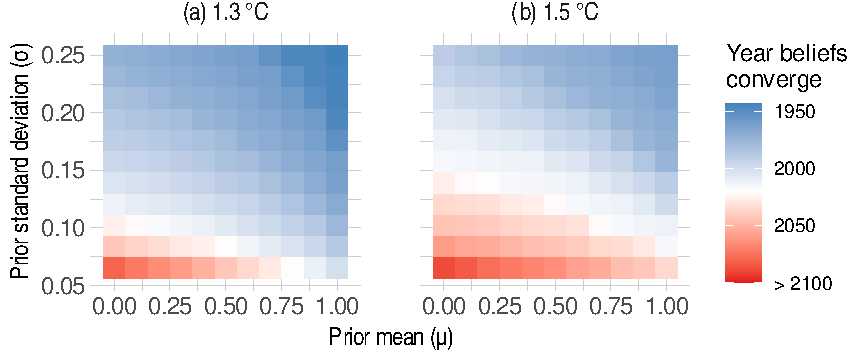
\includegraphics[width=1\linewidth]{/home/grant/Documents/Papers/Sceptic/sceptic-priors/figs/evidence-1} 

}

\caption{When do sceptic beliefs about TCR converge with mainstream estimates? Axes denote the means and standard deviations of a range of normally-distributed sceptic priors on TCR. Convergence is defined as occurring when the mean posterior TCR for a particular prior equals the relevant target value, i.e. (a) 1.3 °C or (b) 1.5 °C. The year of convergence assumes a starting date of 1866 to coincide with the common historical dataset. Blue shading indicates that convergence is feasible with historically available data. Red shading indicates that convergence can only occur once additional data has been accumulated in the future.}\label{fig:evidence}
\end{figure}

An implication of this thought experiment is the following. If someone
is unpersuaded of the human influence on climate today --- despite all
of the available evidence --- then there is a high probability that they
will remain unconvinced for many years hence. The extent to which these
extreme sceptics constitute a meaningful voting block is an open
empirical question. However, it is striking to think that such
individuals are already out of reach from the perspective of
comprehensive climate policy. Even the accumulation of evidence over the
next several decades may not be enough to convince them. Scientific
communication efforts should be tailored appropriately, specifically
targeting moderates for persuasion (e.g.~lukewarmers) rather than
engaging sceptics \emph{en masse}.

\hypertarget{sec:sensitivity}{%
\subsection{Sensitivity analysis}\label{sec:sensitivity}}

\begin{table}

\caption{\label{tab:sens_tab}TCR: Sensitivity analysis and alternative specifications. \label{tab:sensitivity}}
\centering
\begin{threeparttable}
\begin{tabular}[t]{lll}
\toprule
Key & TCR & Comment\\
\midrule
CW14 & 1.6 (1.4, 1.9) & Alternative GMST series.\\
GISTEMP & 1.8 (1.5, 2.0) & Alternative GMST series.\\
HadCRUT ME & 1.6 (1.4, 1.8) & Measurement error in GMST data.\\
DF18 & 1.4 (0.9, 2.6) & Measurement error in forcings data.\\
MEA16 I & 2.2 (1.9, 2.5) & Adjusted forcing efficacies (means).\\
\addlinespace
MEA16 II & 1.9 (-0.7, 3.4) & Adjusted forcing efficacies (distributions).\\
Anthro & 1.6 (1.4, 1.8) & Separate anthropogenic from natural forcings.\\
CO$_2$ & 1.7 (1.3, 2.0) & Separate CO$_2$ from other forcings.\\
\bottomrule
\end{tabular}
\begin{tablenotes}[para]
\item \textit{Notes:} 
\item TCR means are given in °C, with 95\% credible intervals in parentheses. The estimates above are computed using noninformative priors only. Full distributions for all prior types across all sensitivity runs are provided in the Supplementary Material. See main text for additional details.
\end{tablenotes}
\end{threeparttable}
\end{table}

I consider a number of alternative specifications to test the
sensitivity of my findings. Table \ref{tab:sensitivity} summarises the
resulting posterior TCR distributions that obtain under noninformative
priors --- see the Supplementary Material for full posterior
distributions across all prior types. The general effect of these
alternate specifications, regardless of prior, is to nudge the posterior
TCR mean higher. We also see a widening of the posterior distributions,
as some specifications explicitly introduce additional uncertainty into
the estimation.

A first sensitivity check is motivated by the fact that HadCRUT4 is
known to suffer from potential coverage biases due to incomplete
placement of \textit{in situ} thermometers. I therefore rerun the
analysis with two alternate reconstructions of GMST.
\cite{cowtan2014coverage}, hereafter CW14, correct for the gaps in the
HadCRUT4 dataset by using an interpolation algorithm based on the
``kriging'' method. Similarly, the NASA Goddard Institute for Space
Studies uses an extrapolation algorithm to overcome coverage bias in
GISTEMP, its own GMST reconstruction. Running the Bayesian regression
model on these alternative series yields moderately higher TCR values
compared to HadCRUT4. Under a noninformative prior, the posterior TCR
means (and 95\% Bayesian credible intervals) are 1.6 °C (1.4--1.9 °C)
for CW14 and 1.8 °C (1.5--2.0 °C) for GISTEMP. Given that the explicit
goal of this paper is to evaluate policy options from the perspective of
climate sceptics, I continue using the results from the HadCRUT4 series
as a default. Yet, it should be noted that this is a conservative choice
that may, at least marginally, understate the true level of warming.

All three GMST reconstructions also provide estimates of measurement
error. The Bayesian framework is ideally suited to incorporate such
knowledge, since the nested model structure allows us to fully specify
measurement error on the dependent variable within the regression model
itself. Doing so in the present setup yields TCR estimates that are
effectively identical to those presented in Table \ref{tab:regtab},
namely 1.6 °C (1.4--1.8 °C). This is unsurprising once we recall that
measurement error on the dependent variable is absorbed by the
disturbance term of the regression model.\footnote{For example, see
  p.~326 of \cite{greene2007econometric}. To illustrate with a simple
  univariate case: The regression model can be written as
  \(y_t \sim \mathcal{N}(\beta X_t, \sigma^2 + \omega_t^2)\), where
  \(\sigma^2 = \mathop{\mathrm{Var}}(\epsilon)\) is the variance of the
  error term and \(\omega_t^2 = \mathop{\mathrm{Var}}(\nu_t)\) is the
  variance of the measurement error on \(y_t\). Together, \(\epsilon\)
  and \(\nu_t\) make up the overall disturbance of the regression.}
Since the Bayesian regression framework is primarily concerned with
total model uncertainty, specifying the relative contribution of such
measurement error to the overall disturbance doesn't meaningfully alter
the analysis --- though it may be useful for incorporating known sources
of heteroscedasticity.\footnote{See \cite{lewis2005edv} for a related
  discussion in a frequentist setting.} The primary regression results
already have GMST measurement error ``baked in'' to the estimation,
regardless of whether we define it explicitly or not.

The same could not be said for measurement error in the model
explanatory variables --- radiative forcing, most importantly --- which
needs to be accounted for explicitly. Fortunately, the Bayesian
framework offers a natural way to incorporate this type of uncertainty.
I conduct a Monte Carlo simulation using the 1,000-member ensemble of
forcing estimates from \cite{dessler2018ecs}; hereafter DF18.
Specifically, I run my Bayesian regression model on each member of the
DF18 ensemble separately --- 1,000 different regressions with each
taking their corresponding forcings as the true state of the world ---
before aggregating the posterior results into a single meta-distribution
at the end.\footnote{This probabilistic approach is the standard
  Bayesian solution to dealing with measurement error in explanatory
  variables. In contrast, deriving consistent regression estimators when
  there is measurement error in explanatory variables can be a much more
  complicated affair in frequentist settings
  \cite{greene2007econometric}.} The resulting posterior is wider, as
expected due to the additional uncertainty. But the TCR mean and 95\%
credible interval of 1.4 °C (0.9--2.6 °C) are still well situated within
the IPCC ``likely'' range.

Thus far, I have assumed that the different physical drivers that make
up total radiative forcing have the same per-unit effect on GMST.
Forcing agents that yield a similar radiative imbalance in Wm\(^{-2}\)
are expected to result in similar feedbacks and responses in GMST.
However, recent research has suggested that the warming efficacy of
different forcing agents can, in fact, vary with factors like geography.
Aerosol emissions, for example, are primarily concentrated in the
mid-to-high latitudes of the Northern Hemisphere. The disproportionately
large land mass in this region causes aerosol forcing to exhibit
stronger feedback effects and an accelerated temperature response than
if it were uniformly distributed across the globe
\cite{shindell2014tcr}. The implications of such forcing inhomogeneity
on climate sensitivity estimates are more fully explored by
\cite{marvel2016implications}, hereafter MEA16. I adapt their results to
construct an adjusted series of total radiative forcing, where each
forcing agent is pre-multiplied by an appropriate efficacy coefficients
(see Supplementary Material). Specifically, I consider two approaches.
The first takes MEA16's mean efficacy estimates as given and ignores all
modeling uncertainty in their results. The second explicitly accounts
for modeling uncertainty in much the same way that was used to account
for explanatory variable measurement error above; i.e.~I conduct a Monte
Carlo exercise that repeatedly samples from the \emph{t} distributions
underlying each forcing efficacy estimate and then combines the
posterior results from many regressions into a single meta-distribution
at the end. Consistent with MEA16, both approaches lead to a pronounced
increase in the posterior TCR mean, with the Monte Carlo sampling
approach further yielding a much wider credible interval. However, MEA16
note that data artefacts --- e.g.~small changes experienced by some
forcing agents over their study period --- automatically induce large
uncertainties in the associated efficacy estimates. Combined with the
fact that MEA16 obtain their results from a single climate model rather
than a multi-model ensemble, this means that the unusually wide credible
intervals of the latter Monte Carlo approach should be regarded with
caution.

As final sensitivity test, I relax the constraint that all sources of
radiative forcing have to be included in the regression model under the
same composite \(RF\) term. Recall that this decision was motivated by
the fact that the forcing agents in my dataset are all defined in
Wm\(^{-2}\). Separating out individual forcings and then placing
different priors on them will likely cause the model to become
physically inconsistent.\footnote{For the anthropogenic forcings, the
  use of a composite term also avoids introducing severe
  multicollinearity into the econometric estimation.} Such admonishments
notwithstanding, I implement two version of this unphysical model. The
first separates out anthropogenic forcings (e.g.~GHGs) from natural
forcings (e.g.~solar radiation). The second separates out CO\(_2\)
forcing from all other sources. In both cases, the subjective priors
from Table \ref{tab:sceppriors} are placed on the isolated anthropogenic
component, while all other variables take noninformative priors. Both
sets of regressions yield very similar results to the main,
physically-correct specification. If anything, isolating CO\(_2\) on its
own yields a higher posterior TCR for certain prior types. However, this
latter implementation should be treated with caution for reasons
previously described.

\hypertarget{sec:future}{%
\subsection{Future temperatures}\label{sec:future}}

Climate policy is largely predicated upon the risks to future
generations. As such, any policy discussion must consider predictions
that run many years into the future. TCR estimates are one means of
gaining an insight into how global temperatures will evolve over the
coming decades. A more explicit way of demonstrating this is by
predicting temperatures until the end of the century.

While the trajectory of future radiative forcings is subject to much
uncertainty, some guidance is available in the form of the IPCC's
Representative Concentration Pathways \cite{van2011rcp}. These so-called
``RCPs'' describe a family of emissions scenarios, where total
anthropogenic forcings evolves according to various economic,
demographic and technological assumptions. Each RCP includes a core
component of atmospheric CO\(_2\) concentrations, while they all share a
common prediction for radiative forcing due to solar activity. I take
these series as the basis for constructing covariate vectors to predict
temperatures until the year 2100. For the remaining explanatory
variables --- stratospheric aerosols, SOI and AMO --- I take the mean
historical values from my dataset. A summary of covariate vectors in
2100 for each RCP scenario is provided in the Supplementary Material.

Fig. \ref{fig:gmst-pred} shows the temperature evolution for each RCP
under the noninformative case, which I again take as the benchmark. As
discussed in Section \ref{sec:likelihood}, it would be inappropriate to
extrapolate my regression framework to scenarios that are characterised
by significant changes in the rate of radiative forcing. The confounding
effect of (unaccounted for) thermal inertia in the oceans would render
these model predictions ill-conditioned. I therefore focus on RCPs 6.0
and 8.5, which maintain steady rates of forcing increase.\footnote{Temperature
  predictions for RCPs 2.6 and 4.5 --- depicting respective CO\(_2\)
  stabilisation scenarios --- are included in Fig. \ref{fig:gmst-pred}
  for reference purposes only.} The principal message is that CO\(_2\)
concentrations must be constrained to well below RCP 6.0, if we are to
avoid a 2 °C rise in global temperatures. Given the prominence of this
particular threshold in international climate treaties and the popular
narrative, the result is a reinforcement of commonly cited emissions
targets such as 450 and 540 ppmv. On the other hand, we can expect to
breech even 3 °C by the year 2100 if we continue along a truly
unconstrained emissions path à la RCP 8.5.

\begin{figure}

{\centering 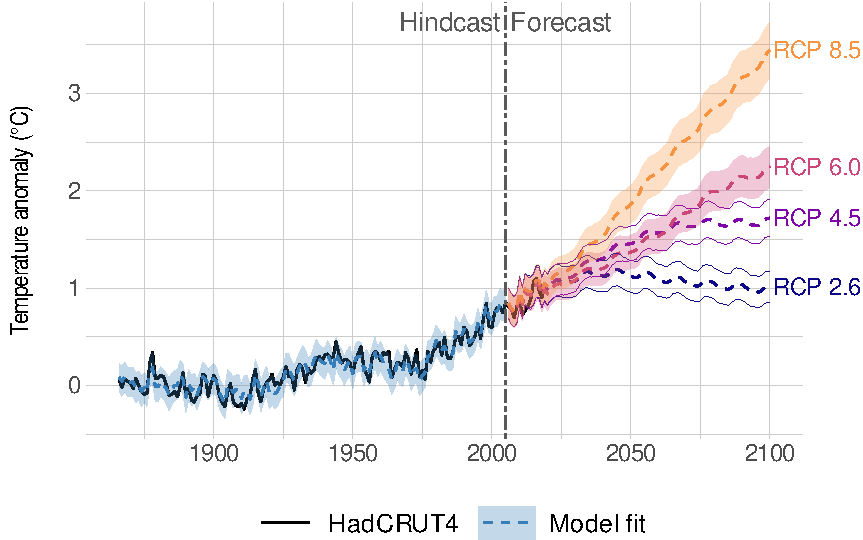
\includegraphics[width=1\linewidth]{/home/grant/Documents/Papers/Sceptic/sceptic-priors/figs/gmst-pred-1} 

}

\caption{Model fit and prediction: noninformative priors. Temperature anomaly relative to the 1871--1900 average. Shaded regions denote 95\% credible intervals. Note that predictions for RCPs 2.6 and 4.5 are potentially ill-conditioned and are included for reference purposes only. See text for details.}\label{fig:gmst-pred}
\end{figure}

What of the predictions yielded by our group of climate sceptics? While
it is straightforward to redraw Fig. \ref{fig:gmst-pred} for each prior
type, a more intuitive comparison can be made by looking at the full
distribution of warming that each sceptic expects by the end of the
century. Fig. \ref{fig:gmst2100} plots the predictive temperature
density in the year 2100 for all prior types by RCP scenarios 6.0 and
8.5. Again, the data have a clear tendency to overwhelm even reasonably
staunch forms of climate scepticism. Nearly all of the stylised sceptics
would expect to breach the 2 °C threshold by 2100 under RCP 6.0, while a
temperature rise of more than 3 °C is likely under under RCP 8.5. An
exception can only be found in the form of the Strong Denier, whose
extreme prior dominates the posterior in a way that obviates nearly all
concern about large temperature increases.

\begin{figure}

{\centering 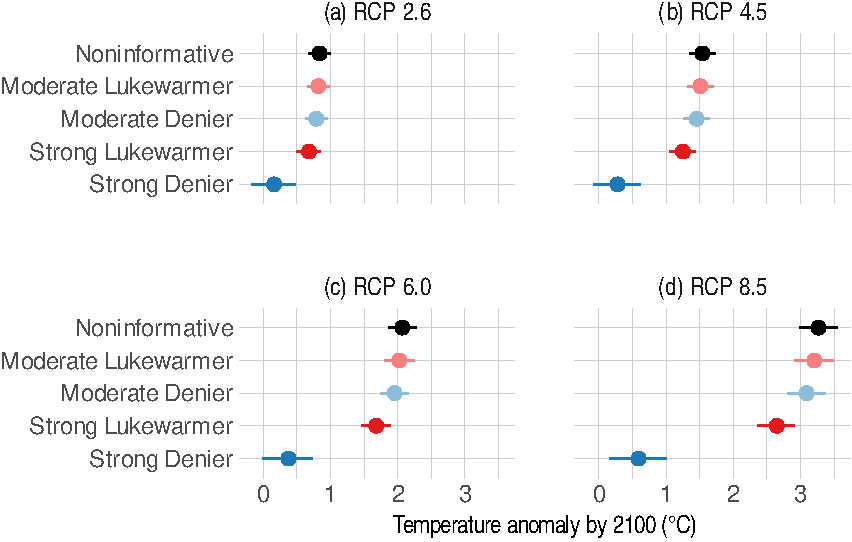
\includegraphics[width=1\linewidth]{/home/grant/Documents/Papers/Sceptic/sceptic-priors/figs/gmst2100-1} 

}

\caption{Predicted temperature anomaly by 2100: all priors types. Points denote means and error bars denote 95\% credible intervals.}\label{fig:gmst2100}
\end{figure}

\hypertarget{sec:welfare}{%
\subsection{Welfare implications and the social cost of
carbon}\label{sec:welfare}}

Provided they consider enough data, we have seen that most climate
sceptics should be able to agree that a 2 °C target requires limiting
CO\(_2\) concentrations to around 540 ppmv. However, whether someone
actually subscribes to policy measures aimed at achieving the 2 °C goal
is dependent on many things; their choice of discount rate, beliefs
about the efficacy of policy, damage expectations, etc. Such issues are
largely beyond the scope of this paper. Nonetheless, we may still gain a
deeper insight into the welfare implications of our posterior TCR values
by analysing their effect on the social cost of carbon (SCC). The SCC
represents the economic costs associated with a marginal unit of
CO\(_2\) emissions. It can therefore be thought of as society's
willingness to pay for the prevention of future damages associated with
human-induced climate change.

Obtaining SCC estimates generally requires the use of integrated
assessment models (IAMs), which are able to solve for optimal climate
policy along a dynamic path by simulating across economic and climate
systems. The PAGE model (\cite{hope2011page09},
\cite{hope2011page09scc}) is ideally suited to our present needs. It is
widely used as one of the major IAMs for evaluating climate policy
(\cite{nordhaus2014scc}, \cite{iwg2016scc}). More importantly, PAGE
accepts random variables as inputs and yields the type of probabilistic
output that is consistent with the rest of this paper. I take the
posterior TCR distributions yielded by my Bayesian regression model and
use these as inputs for calculating the SCC. The PAGE defaults are used
for the remaining parameters.

Table \ref{tab:scc} summarizes the SCC distributions across all prior
groups in 2005 US dollars. The full probability distributions are highly
skewed and characterised by extremely long upper tails (see the
Supplementary Material). This is largely due to the fact that PAGE
allows for the possibility of major disruptions --- e.g.~melting of the
Greenland ice sheet --- at temperatures above 3 °C. Such low
probability, high impact events would yield tremendous economic losses
and result in some extreme SCC values as a consequence. Note too that
the frequency of these events are more common in my adapted version of
PAGE, since I replace the default triangular (i.e.~bounded) TCR
distribution with the posterior TCR distributions from my model. The
latter are approximately normally distributed, thus permitting small but
positive weight in the tails. For this reason, I provide both the mean
and median SCC values alongside the 95\% probability interval.

\begin{table}

\caption{\label{tab:scc_tab}Social cost of carbon (US\$2005 per ton). \label{tab:scc}}
\centering
\begin{threeparttable}
\begin{tabular}[t]{lccc}
\toprule
 & Mean & Median & 95\% Prob. Interval\\
\midrule
Noninformative & 79 & 41 & (12, 168)\\
Moderate Lukewarmer & 65 & 39 & (11, 160)\\
Strong Lukewarmer & 48 & 26 & (7, 107)\\
Moderate Denier & 68 & 36 & (10, 149)\\
Strong Denier & 2 & 1 & (0, 5)\\
\bottomrule
\end{tabular}
\begin{tablenotes}[para]
\item \textit{Notes:} 
\item Results for each agent type are obtained from 10,000 simulation runs of PAGE. Posterior TCR distributions serve as key inputs to the model, while the remaining parameters are set to the PAGE model defaults.
\end{tablenotes}
\end{threeparttable}
\end{table}

Excepting the Strong Denier, the SCC for all prior types is comfortably
larger than zero. The mean value ranges from \$48 to \$79 per ton (2005
prices), while the 95\% probability interval extends from around \$7 to
upwards of \$107 per ton. These results are consistent with the SCC
estimates found within the literature. For example, an influential
synthesis review conducted by the United States government under the
Obama administration established a mean SCC value of \$12--\$62 per
tonne (2007 prices), depending on the preferred discount rate
(\cite{iwg2016scc}). The encouraging point from a policy perspective is
that such congruence exists despite the fact that the analysis proceeds
from an initial position of scepticism. Another way to frame the SCC
estimates presented here is to imagine that each prior type represents
an equal segment of a voting population. We would then expect to see
broad support for a carbon tax of at least \$20--\$25. While such a
thought experiment clearly abstracts from the many complications that
would arise from free-riding and so forth, again we see that nominal
climate scepticism does not correspond to a mechanical dismissal of
climate policy.

\hypertarget{sec:discussion}{%
\section{Discussion}\label{sec:discussion}}

We have seen that a non-trivial carbon price is consistent with a range
of contrarian priors once we allow for updating of beliefs and,
crucially, consider enough of the available data. An optimist might
interpret these findings as a sign that common ground on climate policy
is closer than many people think. On the other hand, they may also help
to explain why the policy debate is so polarised in the first place. As
all intermediate positions are absorbed into the mainstream, only the
most hardcore sceptics will remain wedded to their priors. Such a group
is unlikely to brook any proposals for reduced carbon emissions and
virtually no amount of new information will convince them otherwise.
Taken together with the persistent scepticism that one sees in actual
polling data (e.g.~\cite{saad2019americans}), it then becomes reasonable
to ask whether real-life climate sceptics hold such extreme views? For
that matter, are they numerous or vocal enough to prevent political
action (\cite{lewandowsky2019influence})? Such considerations are
reinforced by the idealized nature of the analysis until now.
Irrespective of the scientific merit of working through such a set-up,
normal people clearly do not update their priors in lockstep with a
Bayesian regression model, supported by large dataset of time-series
observations.

A natural starting point for thinking about these issues is to take a
closer look at the mechanisms underlying posterior agreement formation.
The notion that partisans should converge toward consensus with
increasing information has long been taken as a logical consequence of
Bayes' theorem. Indeed, empirical evidence to the contrary has been
cited as a weakness of the Bayesian paradigm and its relevance to
real-life problems (e.g.~\cite{kahneman1972subjective}). This is a
misconception. Nothing in the Bayesian paradigm precludes the
possibility of diverging opinions in the face of shared information
(\cite{jaynes2003probability}, \cite{bullock2009partisan}). It may even
be the case that the same information has a polarising effect on
individuals, pushing them towards opposite conclusions. This is perhaps
most easily shown by incorporating perceptions of trust and source
credibility into our Bayesian model. In other words, we must broaden our
conception of someone's ``prior'' so that it describes not only their
existing beliefs about some phenomenon \(S\), but also the credibility
that they assign to different sources of information about \(S\).

Consider an example, which is closely adapted from a related discussion
in \cite{jaynes2003probability}. Al, Bob and Christie hold different
beliefs about climate change. Al is a ``warmist'', Bob is a
``lukewarmer'' and Christie is a ``denier''. These labels are
encapsulated by the prior probabilities that each person assigns to
climate sensitivity \(S\), which we assume for simplicity is either high
or low: \(S \in {S_L, S_H}\). Denote by \(I\) an individual's prior
information about the world. Then, indexing by the first letter of their
names, we summarise their prior beliefs about climate change as the
following probabilities: \(P(S_H|I_A)=0.90\), \(P(S_H|I_B)=0.40\), and
\(P(S_H|I_C)=0.10\).

Suppose that the IPCC now publishes its latest assessment report,
wherein it claims that climate sensitivity is high. How do Al, Bob and
Christie respond to this new data, \(D=D_H\)? It turns out that the
answer hinges on the regard that each individual holds for the IPCC
itself. For example, let us say that all three individuals agree the
IPCC would undoubtedly present data supporting a high climate
sensitivity if that were the true state of the world,
i.e.~\(P(D_H|S_H,I_A) = P(D_H|S_H,I_B) = P(D_H|S_H,I_C) = 1.00\).
However, they disagree on whether the IPCC can be trusted to disavow the
high sensitivity hypothesis if the scientific evidence actually
supported a low climate sensitivity. Despite their different beliefs
about climate sensitivity, assume that Al and Christie both regard the
IPCC as an upstanding institution that can be trusted to accurately
represent the science on climate change. In contrast, Bob is dubious
about the motives of the IPCC and believes that the organisation is
willing to lie in advancement of a preconceived agenda. Representing
these beliefs in terms of probabilities, we have
\(P(D_H|S_L,I_A) = 0.05\), \(P(D_H|S_L,I_B) = 0.89\), and
\(P(D_H|S_L,I_C) = 0.05\).

Recovering the posterior beliefs about climate sensitivity for our three
individuals is now a simple matter of modifying Bayes' theorem to
account for each person's relative trust in the IPCC. For Al, we have

\begin{align}
     P(S_H|D_H,I_A) &= \frac{P(D_H|S_H,I_A)P(S_H|I_A)}{P(D_H|S_H,I_A)P(S_H|I_A) + P(D_H|S_L,I_A)P(S_L|I_A)} \notag \\
                                    &= \frac{1.0\times0.9}{1.0\times0.9 + 0.05\times0.1} \notag \\
                                    &\approx 0.98. \notag
\end{align}

Similarly, we obtain posterior probabilities of 0.43 for Bob and 0.69
for Christie.

Taking a step back, Al now believes even more strongly in the high
climate sensitivity hypothesis, having raised his subjective probability
for \(S_H\) from 90\% to 98\%. Christie has experienced a still greater
effect and has updated her subjective probability for \(S_H\) from 10\%
to 69\%. She now attaches a larger probability to the high sensitivity
hypothesis than the low sensitivity alternative. However, the same
cannot be said of Bob, who has not been swayed by the IPCC report in the
slightest. Both his prior and posterior probabilities suggest that
\(S_H\) only has an approximately 40\% chance of being true. Bob's
extreme mistrust has effectively led him to discount the IPCC's high
sensitivity claim in its entirety.

Extending the above framework to account for increasing granularity is
conceptually straightforward. The principal insight remains the same:
Trust is as much a determinant of whether beliefs are amenable to data
--- and whether individuals converge towards consensus --- as the
precision of the data itself. Such an extension seems especially
relevant to the climate change debate given the sense of scientific
distrust that pervades certain segments of society
(\cite{malka2009association}, \cite{gauchat2012politicization},
\cite{leiserowitz2013climategate}, \cite{fiske2014gaining},
\cite{hmielowski2014attack}). Indeed, recent research supports the
notion that distrust of scientists is causing belief polarization about
climate change in some demographic groups, even as scientific evidence
may increase consensus in others (\cite{cook2016rational},
\cite{zhou2016boomerangs}). Similar ``backfire'' effects have been well
documented in other fields (\cite{nyhan2010backfire},
\cite{harris2015bayesian}).

Perhaps the most important feature of generalising the Bayesian
framework in this way is that it offers a bridge between competing
explanations of climate scepticism as a social phenomenon. Whereas the
so-called ``deficit model'' posits a lack of scientific knowledge and
understanding as key drivers of scepticism, advocates of the ``cultural
cognition'' theory argue that group identity and value systems are more
relevant (\cite{kahan2011cultural}, \cite{kahan2012polarizing},
\cite{ranney2016climate}). A Bayesian model that incorporates
perceptions of source credibility is able to accommodate both camps.
Exposure to new scientific evidence can ameliorate a person's
scepticism, but only if their priors allow for it. This includes factors
like cultural identity and whether they cause us to discount some
sources of information more than others.\footnote{While the precise
  theoretical development differs from the framework presented here, I
  would note the closely-related concept of Bayesian networks
  (\cite{pearl2000bayesian}). Indeed, \cite{cook2016rational} use a
  Bayesian network approach in an experimental setting to document
  (rational) belief polarization after individuals are presented with
  evidence about climate change. Mistrust of climate scientists is a
  primary source of the polarization in their study.}

\hypertarget{sec:conclusion}{%
\section{Concluding remarks}\label{sec:conclusion}}

The goal of this paper has been to explore the way in which prior
beliefs affect our responsiveness to information about climate change.
The Bayesian paradigm provides a natural framework and I have proposed a
group of stylised sceptics to embody the degrees of real-world climate
scepticism. The headline finding is that subjective sceptic priors are
generally overwhelmed by the empirical evidence for climate change. Once
they have updated their beliefs in accordance with the available data,
most sceptics demonstrate a clear tendency to congregate towards the
noninformative case that serves as an objective reference point for this
study. My primary regression specification yields a posterior TCR mean
and 95\% credible interval of 1.6 °C (1.4--1.8 °C) under the
noninformative prior. This distribution sits comfortably within the
IPCC's ``likely'' TCR range of 1.0--2.5 °C and is robust to variety of
sensitivity checks. Indeed, accounting for factors that could
conceivably affect the results --- alternate data sources, adjusted
forcing efficacies, measurement error, etc. --- tends to nudge the mean
TCR estimate upwards.

Unsurprisingly, given their congruence with mainstream estimates, I show
that the updated beliefs of various sceptics are generally consistent
with a social cost of carbon of at least US\$25 per ton. Only those with
extreme \emph{a priori} sceptic beliefs would find themselves in
disagreement. Or, feel any confidence in the notion that unfettered
emissions growth will not lead to substantial future warming. This
suggests that a rational climate sceptic, even one that holds relatively
strong prior beliefs to begin with, could embrace policy measures to
constrain CO\(_2\) emissions once they have seen all of the available
data. At the same time, perhaps the most salient finding of this paper
is that belief convergence is a non-linear function of prior strength.
Anyone that remains unconvinced by the available data today is unlikely
to converge with the mainstream consensus for many years hence. Their
implied priors are of such a strength that even decades more of
accumulated evidence may not be enough to convince them. Fully
disentangling the root causes of such information immunity --- whether
climate sceptics are extremely sure of their priors, distrustful of
scientists and other experts, or some combination thereof --- remains an
important area for future research.

\hypertarget{declarations}{%
\section*{Declarations}\label{declarations}}
\addcontentsline{toc}{section}{Declarations}

\begin{itemize}
\item
  \emph{Ethical Approval.} Not applicable.
\item
  \emph{Consent to Participate.} Not applicable.
\item
  \emph{Consent to Publish.} Not applicable.
\item
  \emph{Authors Contributions.} G.R. McDermott is the sole author for
  this article.
\item
  \emph{Funding.} The author has no relevant financial or non-financial
  interests to disclose.
\item
  \emph{Competing Interests.} The author has no conflicts of interest to
  declare that are relevant to the content of this article.
\item
  \emph{Availability of data and materials.} All code and data for this
  article are available at
  \url{https://github.com/grantmcdermott/sceptic-priors}.
\end{itemize}

\bibliographystyle{spphys}
\bibliography{sceptic.bib}

\end{document}
